\documentclass[11pt, a4paper]{article}

\usepackage{graphicx}
\usepackage[a4paper,top=3cm,bottom=2cm,left=2cm,right=2cm,marginparwidth=1.75cm]{geometry}
\usepackage[english]{babel}
\usepackage[utf8x]{inputenc}
\usepackage{subfig}
\usepackage{float}
\usepackage{amsmath}
\usepackage{amssymb}
\usepackage{mhchem}
\usepackage{hyperref}
\usepackage{tikz}
\usepackage{cancel}
\usepackage{bm}

\graphicspath{ {./images} }
\newcommand*{\qed}{\hfill\ensuremath{\quad\square}}%
\newcommand*{\rad}{\ensuremath{\,\text{rad}}}
\newcommand*{\R}{\ensuremath{\mathbb{R}}}
\newcommand*{\C}{\ensuremath{\mathbb{C}}}
\renewcommand*{\Re}{\operatorname{Re}}
\renewcommand*{\Im}{\operatorname{Im}}
\renewcommand*{\epsilon}{\varepsilon}
\renewcommand*{\phi}{\varphi}
\renewcommand*{\d}{\text{d}}

\DeclareRobustCommand{\uvec}[1]{{%
  \ifcat\relax\noexpand#1%
    % it should be a Greek letter
    \bm{\hat{#1}}%
  \else
    \ifcsname uvec#1\endcsname
      \csname uvec#1\endcsname
    \else
      \bm{\hat{\mathbf{#1}}}%
     \fi
   \fi
}}

\makeatletter
\renewcommand*\env@matrix[1][*\c@MaxMatrixCols c]{%
  \hskip -\arraycolsep
  \let\@ifnextchar\new@ifnextchar
  \array{#1}}
\makeatother

\newtheorem{theorem}{Theorem}
\numberwithin{equation}{section}
\numberwithin{figure}{section}

%------------------------------------------------
%Templates for images and figures
% \begin{figure}[h]
%   \centering
%   \subfloat[caption 1]{{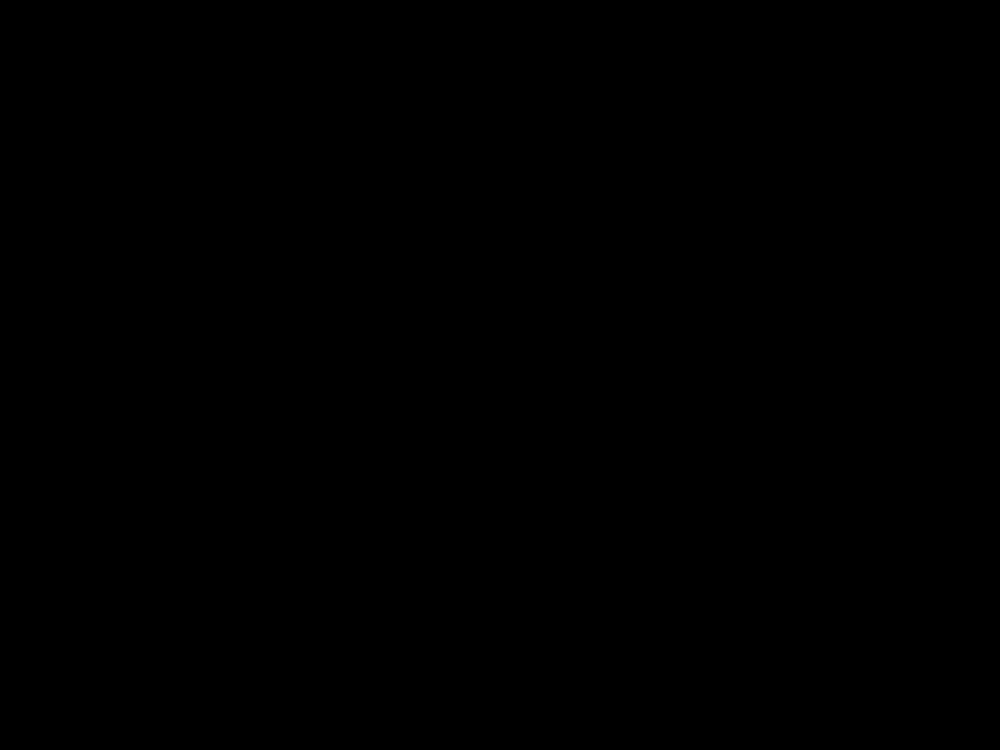
\includegraphics[width=30mm]{images/placeholder.png}}}%
%   \qquad
%   \subfloat[caption 2]{{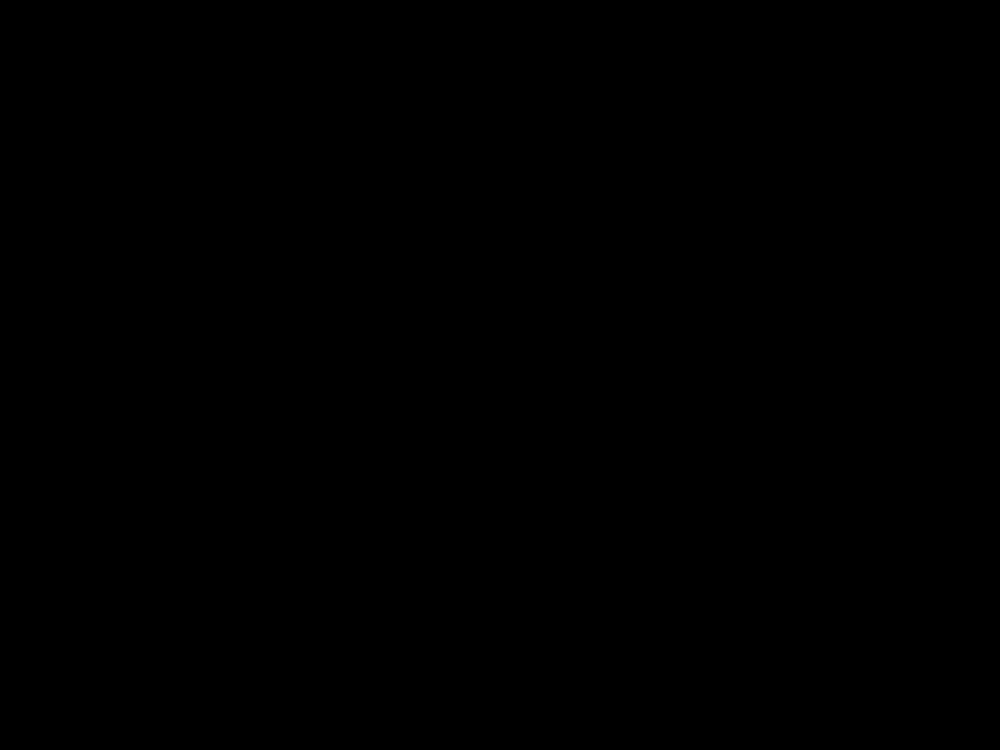
\includegraphics[width=30mm]{images/placeholder.png}}}%
%   \caption{Description}
% \end{figure}

% \begin{figure}[h]
%   \centerline{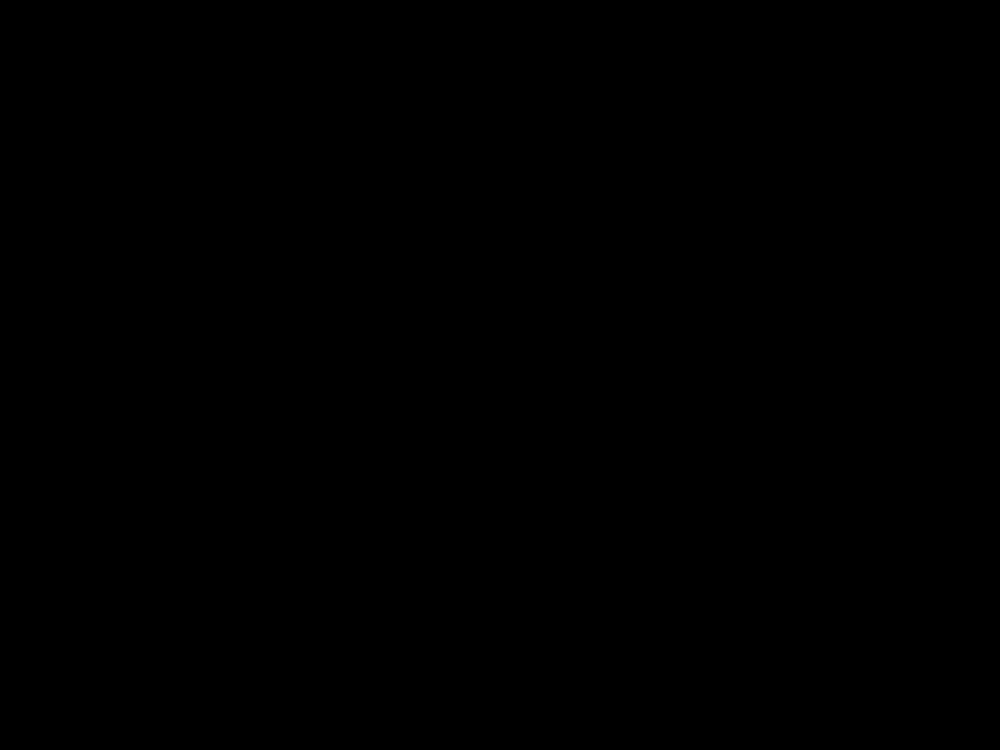
\includegraphics[width=50mm]{images/placeholder.png}}
%   \caption{Description}
% \end{figure}

%Template for a simple table 
%\begin{table}[h]
%   \caption{Description} %title of the table
%   \centering % centering table
%   \begin{tabular}{l rr} % creating three columns
%     \hline\hline %inserting double-line
%     & & \\ [0.5ex] % Insert half line vertical spacing
%     \hline % inserts single-line
%     & & \\ 
%     & & \\
%     & & \\
%     & & \\
%   \hline % inserts single-line
%   \end{tabular}
%   \label{tab:hresult}
% \end{table}
%-----------------------------------------------

\begin{document}
\setcounter{section}{3}

\section{Elasticity}
\subsection{Voigt notation for the stress and strain tensors}
Since the stress and strain tensor are both $3\times 3$ symmetric tensors with 6 unique entries they are often shortened in the form of Voigt notation. The tensor then look like the following:
\begin{align}
  \mathbf{\sigma} &=
  \begin{pmatrix}
    \sigma_{xx} & \sigma_{yy} & \sigma_{zz} & \tau_{xy} & \tau_{yz} & \tau_{zx}\\
  \end{pmatrix}\\
  \mathbf{\epsilon} &= 
  \begin{pmatrix}
    \epsilon_{xx} & \epsilon_{yy} & \epsilon_{zz} & \psi_{xy} & \psi_{yz} & \psi_{zx}\\
  \end{pmatrix}
\end{align}
Where $\mathbf{\sigma}$ is the Cauchy stress tensor and $\mathbf{\epsilon}$ the Green-Lagrange strain tensor.


\subsection{Principal stresses and the relation to eigenvalues}
Recall Mohr's circle from mechanics of materials. There was a state of the stress element where the stress components where in terms of only normal stress and no shear stress. These stresses where called the principal stresses. For a 3D-stress element these principal stresses are given as:
\begin{gather}
  \mathbf{\sigma} \cdot \uvec{n} = \sigma_n \uvec{n}\\
  (\mathbf{\sigma} - \sigma_n I)\uvec{n} = \vec{0}
\end{gather}
Notice that we are looking for a vector which under the transformation of the stress tensor matrix becomes a scaled version of itself. This means $\sigma_n$ is nothing but an eigenvalue of the stress tensor matrix $\mathbf{\sigma}$.


\subsection{Hooke's law and linear elastic behaviour}
The definition for Hooke's law of linear elastic behaviour is given as:
\begin{equation}
  \sigma = E\epsilon
\end{equation}
Where $\sigma$ is the stress, $\epsilon$ the strain and $E$ the Young's module (or sometimes module of elasticity), a material dependent property. This is the case for 1D applications of Hooke's law. When we analyse 3 dimensional elastic behaviour we need to account for transverse contraction in different directions. When material gets longer it also gets thinner. This effect is quantified with Poisson's ratio and is denoted using the letter $\nu$. To simpliify computations we can assume isotropic behaviour for most metals. Isotropic behaviour of material is when the material behaves and deforms the same in all directions. This is fairly accurate when analyzing a crystal structure as you find in steel and other metals, but less accurate for materials like polymers or wood which can behave significantly different parallel to the fibres as oppose to perpendicular to the fibres. The 3D extension of Hooke's law is given as:
\begin{align}
  \epsilon_{xx} &= \frac{\sigma_{xx} - \nu\sigma_{yy} - \nu\sigma_{zz}}{E}\quad& \psi_{xy} = \frac{\tau_{xy}}{G}\\
  \epsilon_{yy} &= \frac{-\nu\sigma_{xx} + \sigma_{yy} - \nu\sigma_{zz}}{E}\quad& \psi_{yz} = \frac{\tau_{yz}}{G}\\
  \epsilon_{zz} &= \frac{-\nu\sigma_{xx} - \nu\sigma_{yy} + \sigma_{zz}}{E}\quad& \psi_{zx} = \frac{\tau_{zx}}{G}
\end{align}
Where $G = \frac{E}{2(1 + \nu)}$. In this case the $\nu\sigma_ii$ terms represent the transverse contraction in the direction of $i$. These terms can then be represented in a $6\times 6$ stiffness matrix $\mathcal{S}$. For isotropic behaviour this matrix is given as:
\begin{equation}
  \mathcal{S} = \frac{E}{(1+\nu)(1-2\nu)}
  \begin{bmatrix}
    1-\nu & \nu   & \nu   & 0               & 0                & 0\\
    \nu   & 1-\nu & \nu   & 0               & 0                & 0\\
    \nu   & \nu   & 1-\nu & 0               & 0                & 0\\
    0     & 0     & 0     & \frac{1-\nu}{2} & 0                & 0\\
    0     & 0     & 0     & 0               &  \frac{1-\nu}{2} & 0\\
    0     & 0     & 0     & 0               &  0               & \frac{1-\nu}{2}
  \end{bmatrix}
\end{equation}
It's inverse is given as:
\begin{equation}
  \mathcal{S}^{-1} = \frac{1}{E}
  \begin{bmatrix}
    1     & -\nu  & -\nu  & 0        & 0         & 0\\
    -\nu  & 1     & -\nu  & 0        & 0         & 0\\
    -\nu  & -\nu  & 1     & 0        & 0         & 0\\
    0     & 0     & 0     & 2(1+\nu) & 0         & 0\\
    0     & 0     & 0     & 0        &  2(1+\nu) & 0\\
    0     & 0     & 0     & 0        &  0        & 2(1+\nu)
  \end{bmatrix}
\end{equation}
We can then use this to express Hooke's Law in matrix form using the Cauchy stress tensor and Green-Lagrange strain tensor:
\begin{gather}
  \mathbf{\sigma} = \mathcal{S}\mathbf{\epsilon}\\
  \mathbf{\epsilon} = \mathcal{S}^{-1} \mathbf{\sigma}
\end{gather}
In the case of anisotropic material behaviour all the individual terms of the stiffness matrix will need to be specified. Because the matrix is symmetric $\mathcal{S}_{ij} = \mathcal{S}_{ji}$, thus the matrix has a total of $13$ indpenedent constants that need to be defined. The stiffness matrix is then given as:
\begin{equation}
  \mathcal{S} =
  \begin{bmatrix}
    \mathcal{S}_{11} & \mathcal{S}_{12} & \mathcal{S}_{13} & 0                & 0                 & 0\\
    \mathcal{S}_{21} & \mathcal{S}_{22} & \mathcal{S}_{23} & 0                & 0                 & 0\\
    \mathcal{S}_{31} & \mathcal{S}_{32} & \mathcal{S}_{33} & 0                & 0                 & 0\\
    0                & 0                & 0                & \mathcal{S}_{44} & 0                 & 0\\
    0                & 0                & 0                & 0                 & \mathcal{S}_{55} & 0\\
    0                & 0                & 0                & 0                 & 0                & \mathcal{S}_{66}
  \end{bmatrix}
\end{equation}
\end{document}